\section{Design af Controller}

Det endelige mål med kontrolsystemet er, at kunne styre orienteringen af rammerne præcist ved at give et vinkel-input. Dette input konverteres så til et fejlsignal, som er forskellen imellem den ønskede vinkel og den faktiske vinkel, som systemet står i. Controllerens opgave er så, at holde øje med fejlen og derigennem beregne sig til en passende PWM duty cycle, så input og output til sidst stemmer overens. 

\begin{figure}[ht]
	\begin{center}
		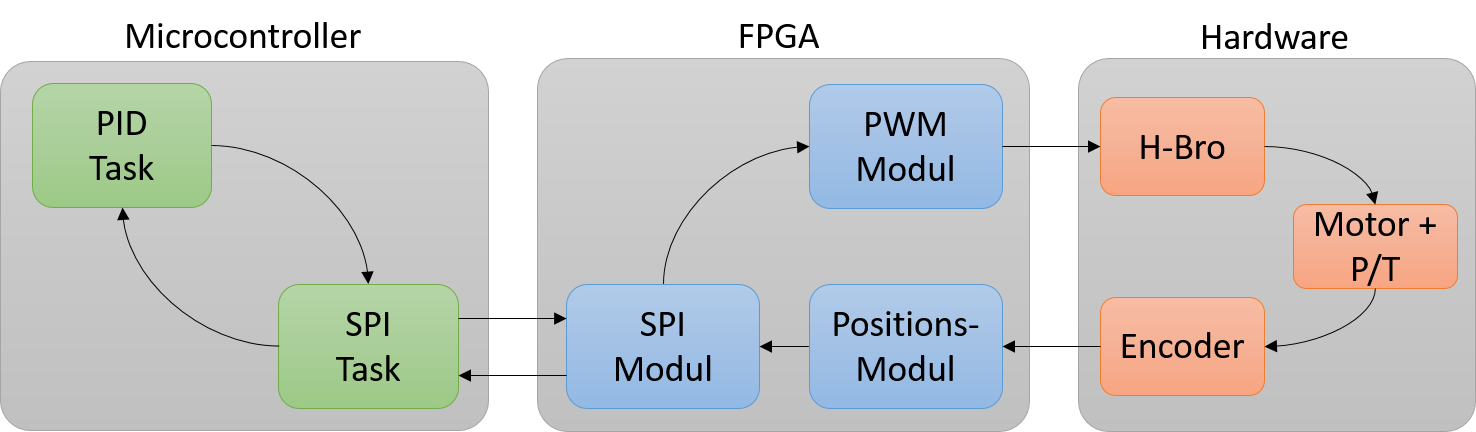
\includegraphics[scale=0.5]{Billeder/Controller_Blok.png}
	\end{center}
\caption{Her ses data flowet for kontrolløkken.}
\label{fig:Blok_Model}
\end{figure}

På figur \ref{fig:Blok_Model} kan man se de vigtigste elementer i kontrolløkken fra microcontrolleren og ud til selve systemet. Ud fra et modelleringsperspektiv er de fire mest interessante dele af systemet som følger:

\begin{itemize}
\item \textbf{H-bro}: Sørger for at regulere forsyningsspændingen på 12V til motoren alt afhængig af den duty cycle som PWM-modulet sender ud. Duty cycle styrer den gennemsnitlige spænding over motorterminalerne. H-broen kan også vende strømmen igennem motoren for at skifte omdrejningsretningen.
\item \textbf{Motor og Pan/Tilt-system}: Producerer en omdrejningshastighed, som er relateret til spændingen over motorterminalerne ved overføringsfunktionen beskrevet i ligning (\ref{eq:tf_pan_tilt}).
\item \textbf{Encoder og Positionsmodul}: To hall sensorer i encoderen genererer pulser, der gør det muligt at bestemme omdrejningsretningen for motoren. Positionsmodulet sørger for at holde styr på pulserne, for at afkode hvilken position motoren har stillet sig i. Dette er muligt hvis man starter med at have en fast reference man tæller fra.
\item \textbf{Controller}: Sørger for at generere et passende PWM-signal, så motoren kan flytte rammerne over i den ønskede position. Dette skal foregå på en måde, så designmålene for projektet overholdes.
\end{itemize}

Modelleringen af systemet viste at motoren og pan/tilt-systemet kunne approksimeres nogenlunde som et 1.-ordenssystem (se ligning \eqref{eq:tf_pan_tilt}).
Hvis man tager udgangspunkt i grey box-modellen af systemet, kan man lave et closed-loop-system, der ser ud som på figur \ref{fig:GB_Model}. På denne model er H-broen modelleret som et gain på 12. PWM-signalet kan variere fra $-1$ til $1$. Encoderen og positionsmodulet fungerer i praksis lidt som en integrator i den forstand at alle ticks summeres op og giver en relativ position. Der er ikke noget gain igennem feedback-løkken da set point'et til controlleren også opgives i ticks. Det vides på forhånd at et tick svarer til $1/3$ af en grad (Se reference i afsnit \ref{subsec:TicksToDeg}), så for at holde kontrolsystemet simpelt, foretages den omregning inden set point'et gives til controlleren. På den måde skal controlleren kun regne i ticks.

\begin{figure}[ht]
	\begin{center}
		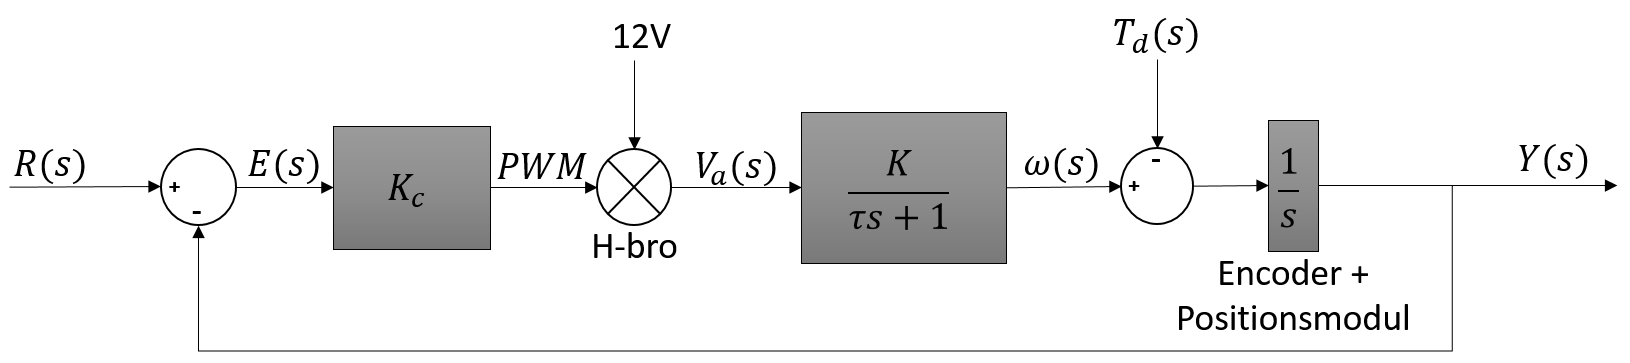
\includegraphics[scale=0.5]{Billeder/Control_Loop.PNG}
	\end{center}
\caption{Closed-Loop kontrolsystem til grey box-modellen}
\label{fig:GB_Model}
\end{figure}

Blokdiagrammet på figur \ref{fig:GB_Model} kan koges ned til overføringsfunktionen beskrevet i (\ref{eq:GB_tf}). Her er H-broen forsimplet til et gain på 12, under den antagelse at PWM-signalet varierer fra $-1$ til $1$.

\begin{equation}\label{eq:GB_tf}
Y(s)=R(s)\frac{12K_{c}K}{s(\tau s+1)+12K_{c}K}-T_{d}(s)\frac{\tau s+1}{s(\tau s+1)+12K_{c}K}
\end{equation}

\subsection{Designmål}

\begin{itemize}

\item Steady state fejl på 0
\item Overshoot $<$ 5 $\%$ XXXX
\item Settling time $<$ 5 sekunder 

\end{itemize}

\subsection{2.-ordenssystem}

Når man designer en controller, kan det være praktisk at approksimere hele systemet som et ideelt 2-ordens-system (ligning \eqref{eq:SO_system}). Disse systemer er meget veldefinerede og forholdsvis lette at beregne på. Parametre som overshoot, settling time, rise time m.m. kan beregnes analytisk og kan give et godt udgangspunkt til ens valg af controller. $\omega_{n}$ er systemets naturlige frekvens og $\zeta$ er systemets damping ratio - jo større en damping ratio, jo bedre en dæmpning af systemets respons har man.

\begin{equation}\label{eq:SO_system}
Y(s)=\frac{\omega_{n}^2}{s^2+2\zeta\omega_{n}s+\omega_{n}^2}
\end{equation}

Hele ideen med at benytte et 2-ordens-system til den indledende analyse, er at man kan finde de områder i s-planet, hvor systemet vil holde sig inden for designmålene, så længe systemets poler placeres der. Disse antagelser gælder naturligvis kun præcist for et 2-ordens-system uden nuller, men det kan sagtens være en udemærket approksimering, hvis man har et system af højere orden med to dominante poler der ligger tæt på $j\omega$-aksen. Som tommelfinger-regel kan man godt tillade sig at kalde to poler for dominante, hvis de er 5 gange tættere på den imaginære akse end resten af polerne. Grunden til at man kigger mest på de dominante poler, er at jo længere man kommer væk fra $j\omega$-aksen jo hurtigere aftager effekten på systemet fra polerne over tid. Derfor ender det med at være de langsomme poler, der dominerer systemets respons.

\begin{figure}[!ht]
	\centering
	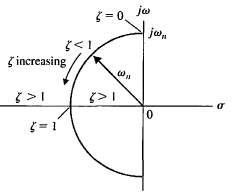
\includegraphics[scale=0.5]{Billeder/Damping_Ratio.PNG}
	\caption{Her kan man se hvordan damping ratio og den naturlige frekvens påvirker polernes placering i et 2-ordens-system.}
	\label{fig:SO_system}
\end{figure}

På figur \ref{fig:SO_system} kan man se hvordan man, alene ud fra polernes placering, kan beskrive en masse om damping ratio og den naturlige frekvens. En ting der ikke fremgår af figuren, er at damping ratio også fortæller noget om, om polerne er komplekse konjugerede eller reelle. Hvis $1>\zeta>0$ er polerne komplekse; hvis $\zeta=1$ ligger der to reelle poler oven i hinanden; hvis $\zeta>1$ er polerne reelle og unikke. Disse tre situationer bliver også ofte beskrevet som henholdsvis underdæmpet, kritisk dæmpet og overdæmpet.




\subsubsection{Steady State Fejl}

For at undersøge om systemet kan drive fejlen i 0, er det nødvendigt at finde et udtryk for $E(s)$, som kan ses på figur \ref{fig:GB_Model}, og ved hjælp af \textit{Final Value Theorem} (\ref{eq:FVT}), finde ud af hvad der er tilbage, når systemet går i steady state. $E(s)$ kan fra blokdiagrammet på figur (\ref{eq:GB_tf}).

\begin{equation} \label{eq:FVT}
lim_{t \to \infty} f(t) = lim_{s \to 0} sF(s)
\end{equation}

\begin{equation} \label{eq:ess}
E(s)=R(s)\frac{s(\tau s+1)}{s(\tau s+1)+12K_{c}K}-T_{d}(s)\frac{\tau s+1}{s(\tau s+1)+12K_{c}K}
\end{equation}

Ved et step-input ($R(s)=A/s$) bliver fejlen drevet i 0, så længe der ikke er nogen disturbance ($T_{d}=0$). Til gengæld vil der, lige så snart der er en disturbance til stede, være en steady state fejl. I ligning (\ref{eq:td_ess}) kan man se resultatet af et disturbance step-input ($T_{d}=A/s$). I virkeligheden vil man kunne se ubalance i tilt-systemet, for eksempel som en step-disturbance.

Hvis man monterer ekstra vægt og flytter tyngdepunktet væk fra rotationsaksen, vil tyngdekraften modarbejde systemet i nogle positioner og hjælpe systemet i andre. Denne ubalance tilføjer et nyt kraftmoment, der påvirker systemet og kan også godt ses som en ny vinkelhastighed, som det er modelleret i figur \ref{fig:GB_Model}.

\begin{equation}\label{eq:td_ess}
e_{ss}=lim_{s \to 0} sE(s)=-\frac{A}{12K_{c}K}
\end{equation}

Det kan altså konkluderes, at man er nødt til at have mindst en integrator i controlleren ($K_{c}$), for at opfylde kriteriet om en steady state-fejl på 0. Ved et ramp-input skal der bruges to integratorer, men det er ikke så interessant for dette projekt, da det kun er forholdsvist langsomme objekter der skal følges. Systemet vil, under normale forhold, kun skulle flytte sig fra et punkt til et andet og falde til ro der. Det vil meget sjældent være nødvendigt for systemet at skulle flytte sig kontinuerligt.

\subsubsection{Overshoot}

Percent Overshoot (P.O.) er defineret som den procentdel systemets største respons afviger fra den ønskede værdi. Dette er et udtryk for, hvor meget systemet skyder forbi målet, når det påvirkes af et step input. Ved hjælp af lidt algebra, differentiering og et par laplace-transformeringer, kan man udlede ligning (\ref{eq:P.O.}) fra (\ref{eq:SO_system} XXXX sidetal i bog) (se Modern Control Systems\cite{ModernControlSystem}), og på den måde finde ud af, hvor meget overshoot systemet har udelukkende ud fra damping ratio. En anden måde at se på problemet, er at man, ved at finde $\zeta$ til et bestemt overshoot, også kan finde den vinkel til de komplekse polers placering, hvor man får netop den mængde overshoot - store vinkler giver stort overshoot og omvendt (se figur \ref{fig:SO_system}). Man kan altså ud fra denne udregning definere et klart område, hvor alle polplaceringer vil opfylde ens krav til overshoot. 

\begin{equation}\label{eq:P.O.}
P.O.=100*e^{-\dfrac{\zeta\pi}{\sqrt{1-\zeta^2}}}
\end{equation}

For at få 5 $\%$ overshoot eller derunder kan det beregnes at $\zeta$ skal være større end 0.690. Det vil sige at polerne skal placeres indenfor det skraverede område på figur \ref{fig:Overshoot} for at opfylde designmålene. Det er værd at nævne igen, at dette kun viser opførslen for et 2-ordens-system, så man kan ikke præcist beskrive opførslen for vores system på denne måde, da det er et 3.ordenssystem med flere nuller. Til gengæld kan man, hvis man tænker sig om under controller-designet, komme meget tæt på. Det er dog stadigvæk smart at vælge polplaceringer med en god margen op til grænseværdien for at være på den sikre side.

\begin{figure}[ht]
	\begin{center}
		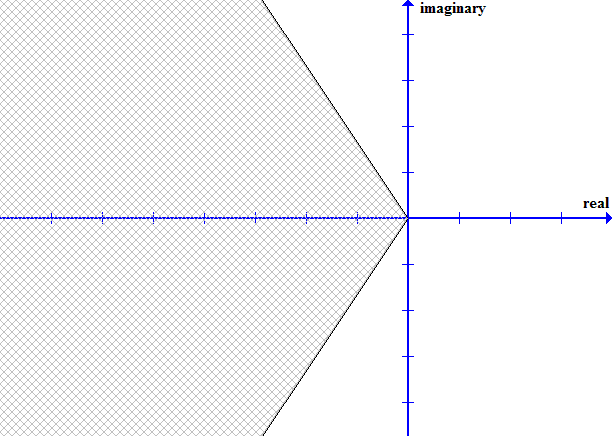
\includegraphics[width=0.8\textwidth]{Billeder/Overshoot.PNG}
	\end{center}
\caption{Det skraverede område viser alle punkter med en $\zeta$-værdi over 0.690. Denne værdi svarer også til en vinkel til den reelle akse på 46.37 grader til begge sider}
\label{fig:Overshoot}
\end{figure}

\subsubsection{Settling Time}

Settling time er defineret som den tid det tager systemet at falde til ro, inden for 2 procent af den ønskede værdi. Hvis man kigger på formlen for impulsresponsen (ligning \ref{eq:impulse_response})  til et 2-ordens-system i tidsdomænet, kan det ses at den dæmpende faktor for systemet er $e^{-\zeta\omega_{n}t}$. Settling time kan derfor beskrives ved $e^{-\zeta\omega_{n}T_{s}}<0.02$ og herfra kan man udlede ligning (\ref{eq:settling_time}).

\begin{equation}\label{eq:impulse_response}
y(t)=\frac{\omega_{n}}{\beta}e^{-\zeta\omega_{n}t}Sin(\omega_{n}\beta t)
\end{equation}

\begin{figure}[ht]
	\begin{center}
		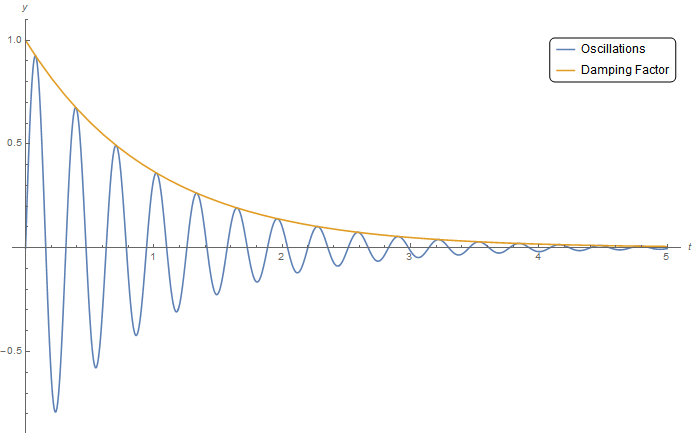
\includegraphics[scale=0.45]{Billeder/Damped_Oscillations.png}
	\end{center}
\caption{Her kan man se hvordan en eksponentiel dæmpende faktor vil påvirke svingninger.}
\label{fig:Damped_Oscillations}
\end{figure}

\begin{equation}\label{eq:settling_time}
T_{s}=\frac{4}{\omega_{n}\zeta}
\end{equation}

For at få en settling time på under $5s$ kan det ud fra ligning \eqref{eq:settling_time} bestemmes at $\omega_{n}\zeta > 0.8$. Det vil med andre ord sige at polerne skal befinde sig til venstre for -0.8 - her refereres der igen til figur \ref{fig:SO_system}. Ligesom det var tilfældet for overshoot-kriterierne, er det også her en god ide at vælge sine poler med en god margen til grænseværdien.

\subsubsection{Delkonklusion}

For at overholde designmålene vedrørende settling time, overshoot og steady state fejl, kan det følgende konkluderes:

\begin{itemize}
\item Damping ratio for et 2.-ordenssystem skal være større end $0.690$.
\item Produktet $\omega_{n}\zeta$ for et 2.-ordenssystem skal være større end $0.8$. Dette produkt svarer til den reelle komponent af to komplekse poler.
\item For at holde steady state fejlen i 0, skal man have en controller med et integrator led. Derfor skal det undersøges hvordan en I-, ID-, PI- og PID-controller påvirker systemet. P- og PD-controllere ignoreres pga af kravet til steady state fejlen.
\end{itemize}

Grænserne skal ses som et absolut minimumskrav, da systemet ikke er et ideelt 2.ordenssystem. Der skal helst være en god margen.

\subsection{Controller-typer}

I denne sektion vil det blive undersøgt, hvilke forskellige controller-typer (I, ID, PI og PID), der bedst kan opfylde projektets krav. Der vil blive set bort fra P- og PD-controllere, da der ønskes en steady state fejl på 0. 

\subsubsection{I Controller}

En I-controller er et integrator-led med et gain. Integratoren svarer til at placere endnu en pol i origo. For at undersøge hvordan denne controller vil opføre sig, kan man bruge root locus metoden for at se, hvordan polerne flytter sig, når controller-gainet øges. 

\begin{equation}\label{eq:I_OpenLoop}
Y(s)=K_{I}\cdot\frac{1}{s}\cdot\frac{12K}{s(s\tau+1)}
\end{equation}

For at plotte root locus i matlab skal man bare bruge open loop overføringsfunktionen (ligning \ref{eq:I_OpenLoop}). På figur \ref{fig:I_rlocus} ses det med al tydelighed at systemet aldrig bliver stabilt med en I-controller, da polerne ikke kan trækkes over på den negative side af $j\omega$-aksen. Af denne grund kan en ren I-controller ikke bruges.

\begin{figure}[t!]
    \centering
    \begin{subfigure}[t]{0.49\textwidth}
     \centering
        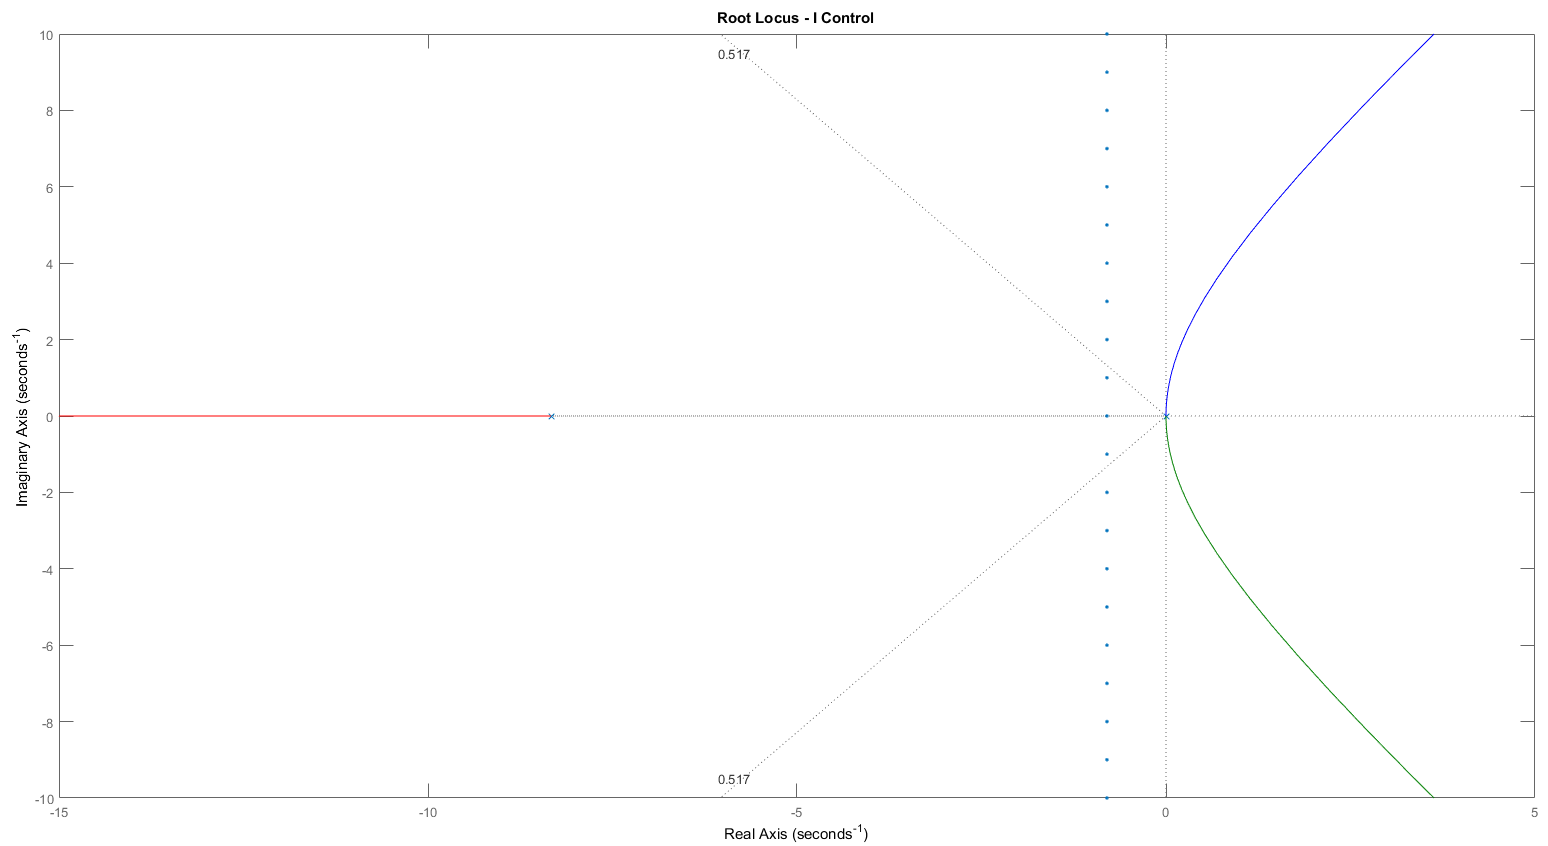
\includegraphics[width=1\textwidth]{Billeder/I_rlocus.PNG}
        \caption{Her ses root locus plottet for vores system med en ID-controller.}
        \label{fig:I_rlocus}
    \end{subfigure}
    \begin{subfigure}[t]{0.49\textwidth}
     \centering
        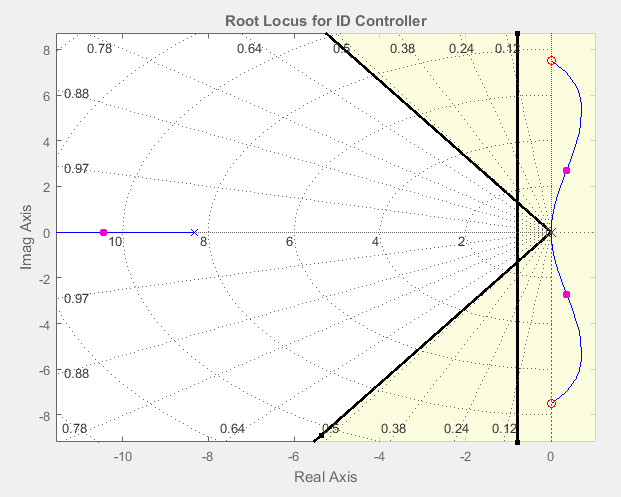
\includegraphics[width=1\textwidth]{Billeder/ID_rlocus.PNG}
        \caption{Her ses root locus plottet for vores system med en I-controller. Det er tydeligt at systemet aldrig kan stabiliseres med et gain alene. Dette plot er lavet med en tidskonstant på 0.12 sekunder, hvilket vil svare til en pol i -8.33.}
        \label{fig:ID_rlocus}
    \end{subfigure}
    \caption{Her ses root locus plottet for vores system med en ID-controller og I-controller.}
\end{figure}

\subsubsection{ID Controller}

ID-controlleren tilføjer to nuller til systemet (\ref{eq:ID_OpenLoop}). Hvis man solver for de to nuller vil man se at de altid ligger på $j\omega$-aksen (\ref{eq:quad}).

\begin{equation}\label{eq:ID_OpenLoop}
Y(s)=\frac{K_{D}s^2+K_{I}}{s}\cdot\frac{12K}{s(s\tau+1)}
\end{equation}

\begin{equation}\label{eq:quad}
\dfrac{0\pm\sqrt{0-4K_{D}K_{I}}}{2K_{D}}
\end{equation}

Denne controller kan heller ikke bruges, da ingen af de to branches fra polerne i origo nogensinde kommer over på den venstre side af den imaginære akse (se figur \ref{fig:ID_rlocus}).

\subsubsection{PI Controller}

En PI controller har også en proportionel del, der summeres med integratoren. Det resulterer i praksis i at der, udover polen i origo fra integratoren, også tilføjes et nul på ventstre side af den imaginære akse. Nullets placering bestemmes af forholdet imellem $K_{I}$ og $K_{P}$.

\begin{equation}\label{eq:PI_OpenLoop}
Y(s)=\frac{K_{P}s+K_{I}}{s}\cdot\frac{12K}{s(s\tau+1)}
\end{equation}

Ud fra root locus beregninger kan det bevises at nullets placering skal ligge til højre for $-0.93$ for at de to branches fra polerne i origo mødes på den reelle akse. (XXXX Skal beviset udpensles med ligninger eller er det fint bare at sige det passer?). $K_{P}$ skal med andre ord helst være større end $K_{I}$. Til gengæld må $K_{P}$ heller ikke blive for meget større end $K_{I}$ (knap $2.6$ gange) fordi det gør systemet for langsomt, da break-in punktet kommer til at ligge på den forkerte side af $0.8$, som er $\omega_{n}\zeta$-grænsen for en settling time under 5 sekunder. 

XXXX figur her.


\subsubsection{PID Controller}

\begin{equation}\label{eq:PID_OpenLoop}
Y(s)=\frac{K_{P}s+K_{I}+K_{D}s^2}{s}\cdot\frac{12K}{s(s\tau+1)}
\end{equation}


XXXX tættere eller længere væk fra model?

Med PI-controlleren er margenen for P- og I-konstanterne og gainet ret snæver, hvis projektets designmål skal overholdes. PID-controlleren giver lidt mere råderum, men man tager også et skridt længere væk fra den ideelle 2.-ordensmodel. Differentieringsledet D tilføjer nemlig et ekstra nul til ligningen. Med to nuller er der ikke længere to branches, der går mod (XXXX reference til figur PI) uendelig langs en lodret asymptote når gainet øges. Der er nu kun en branch der går mod minus uendelig, og det foregår langs den reelle akse. Dette har tre klare fordele:

\begin{itemize}
	\item 	En af polerne fra det modellerede 3-ordens-system glider væk fra de to andre poler ved højere gain. På den måde kan man lettere negligere effekten fra den i modellen. Dette bringer os tættere på 2.ordensmodellen.
	\item  	Man kan altid sørge for at de to dominante poler befinder sig på den 				   	reelle akse (mindre overshoot), hvis de to tilføjede nuller også er reelle og gainet er tilpas stort. 
	\item  	Man kan få de to dominante poler længere væk fra den imaginære akse 					(hurtigere settling time).
\end{itemize}

I de root locus-plots der har være vist indtil videre, har der været brugt en tidskonstant på 0.12 sekunder - denne værdi stammer fra tidlige forsøg på tilt-systemet. Med denne tidskonstant får man en pol på $-1/0.12=-8.33$. Hvis begge nuller placeres til højre for $-8.33$ vil den ene branch følge den reelle akse til venstre for $-8.33$ mod uendelig. På den måde kan man, med et forholdsvist lille gain, skubbe closed-loop-polen fra tidskonstanten så langt ud ad den reelle akse, at den ikke har nogen stor indflydelse på systemet. Det kan også lade sig gøre, hvis et af nullerne eller begge to er til venstre for $-8.33$, det kræver bare et noget større gain.

\begin{figure}[ht]
	\begin{center}
		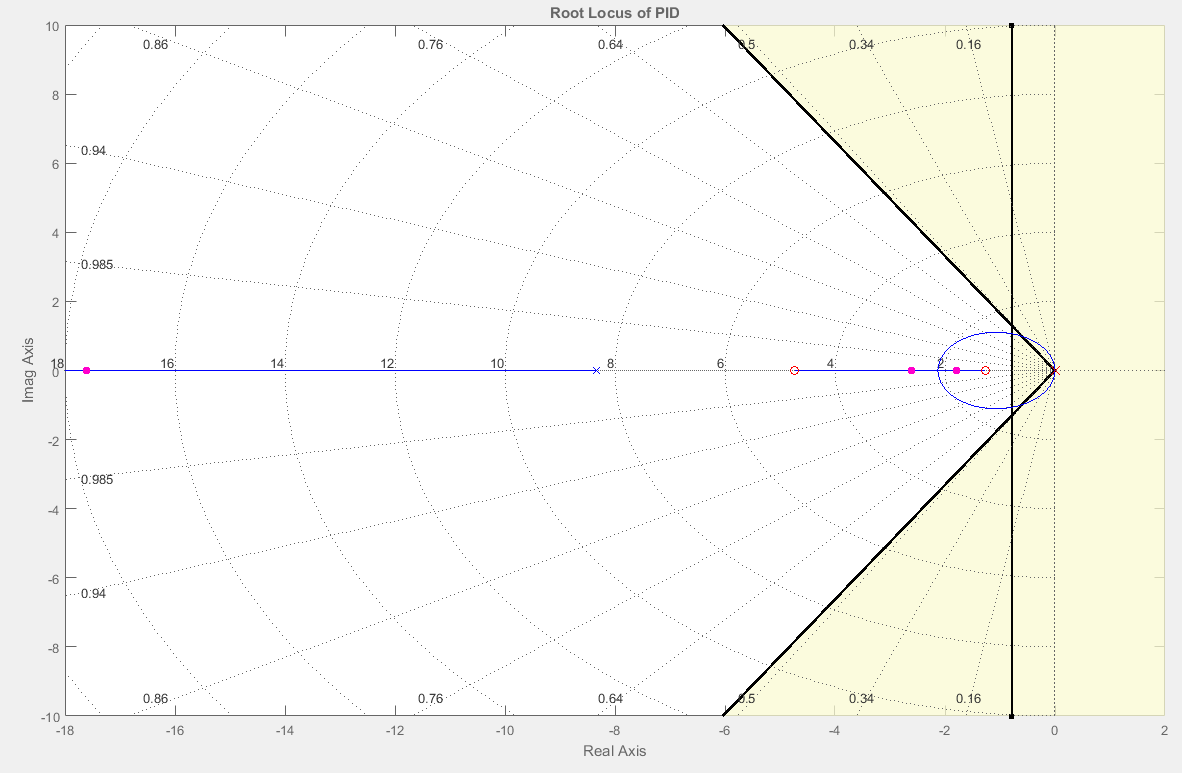
\includegraphics[scale=0.45]{Billeder/PID_rlocus.PNG}
	\end{center}
\caption{Her ses root locus plottet for vores tilt-system med en PID-controller med $K_{P}=6$, $K_{I}=6$, $K_{D}=1$ og et gain på 0.0027}
\label{fig:PID_rlocus}
\end{figure}

\subsection{Delkonklusion}

Det endelige valg af controller falder på PID, da det er den mest fleksible controller i den forstand, at man kan manipulere step responsen meget mere i den retning der ønskes.

%PI-controlleren kan også opfylde projektets designmål, men det er et meget snævert område polerne skal placeres i for det kan lade sig gøre. Med tanke på at controllerens implementering ikke er ideel og at de faktiske system ikke er et 2.-ordenssystem, så giver det ikke mening at vælge PI-controlleren, når man kan designe en PID-controller, der kan placere closed-loop polerne mere solidt i det sikre område. I- og ID-controlleren er ikke en mulighed, da den gør systemet ustabilt.

\subsection{Endeligt Controller design}

For at bestemme den endelige controller til systemet, laves der root locus plots til både pan- og tilt-systemet. Afsnit \ref{sec:Pan_Response} viser at der er ret stor forskel på de to systemer - derfor skal de have hver deres tilpassede controller.

\subsubsection{Tilt-system}

Controlleren til tilt-systemet designes efter at kameraet skal være monteret. Med denne konfiguration fås en tidskonstant på 130 ms og et DC-gain på 605. DC-gain'et er resultatet af outputtet fra controlleren ganget med 12, som er gainet fra H-broen (se figur \ref{fig:Blok_Model}). så $K=605/12$. Dette giver en overføringsfunktion for tilt-systemet som kan ses i ligning (\ref{eq:tilt_tf}). 

\begin{equation}\label{eq:tilt_tf}
\frac{\omega(s)}{V_{a}(s)}=\frac{605/12}{0.13s+1}
\end{equation}

Ud fra ovenstånde ligning kan open loop overføringsfunktionen nu findes. Denne overføringsfunktion ligning \eqref{eq:tilt_ol_tf} kan bruges til at lave de root locus plots som PID-konstanterne designes efter.

\begin{equation}\label{eq:tilt_ol_tf}
\frac{Y(s)}{R(s)}=\frac{K_{P}s+K_{I}+K_{D}s^2}{s}\cdot\frac{605}{s(0.13s+1)}
\end{equation}

Som beskrevet tidligere, kan man se på PID-controlleren som to nuller og en pol i origo. Ved at placere de to nuller i et værktøj som rltool fra matlab kan man aflæse konstanterne direkte. Hvis begge nuller placeres på højre side af den ene open loop pol ($-1/0.13=-7.69$), vil closed loop polen der originere fra den, bevæge sig til venstre mod uendelig, som man også kan se på figur \ref{fig:PID_rlocus}. Derfor er strategien at finde to placeringer til nullerne til højre for $-7.69$, der trækker closed loop polerne, der kommer fra origo, ned mod den reelle akse når gainet øges. På den måde kan alle closed loop poler let placeres indenfor det definerede område fra analysen af 2.ordenssystemer, og jo større gainet bliver, jo længere vil den tredje pol bevæge sig væk fra de to andre.

Med denne metode har man en masse frihed til at vælge PID-konstanterne og samtidig få et respons, der opfylder projektets mål. Det vil sige at der er mange mulige løsninger, så ved at eksperimentere en smule med placeringerne, mens man holder øje med step responsen (igen er rltool et meget nyttigt redskab), kan man finde de konstanter, der bedst opfylder kravene. En af de løsninger der gav de bedste resultater var ved at placere to nuller i $s=-4$. Det giver formlen $(s+4)^2=s^2+8s+16$ som kan aflæses til konstanterne $K_{P}=8$, $K_{I}=16$ og $K_{D}=1$. 

\begin{figure}[ht]
	\begin{center}
		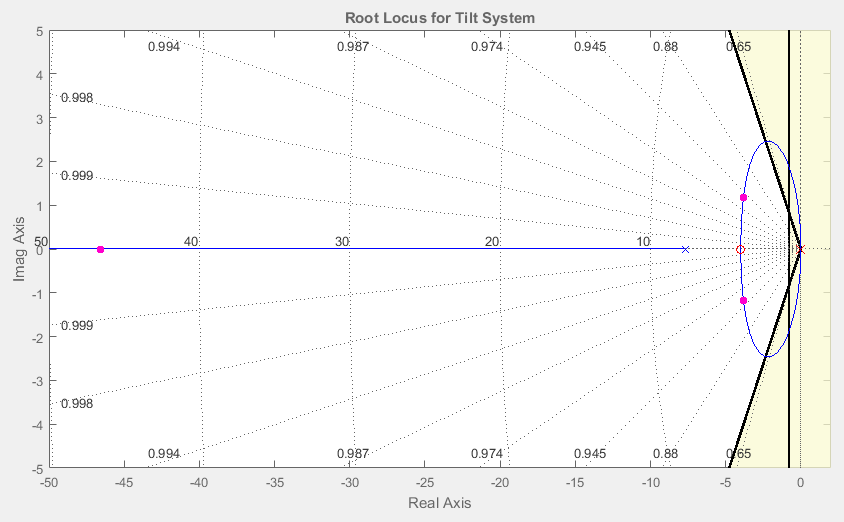
\includegraphics[scale=0.45]{Billeder/Tilt_Rlocus.PNG}
	\end{center}
\caption{Her ses root locus plottet for vores tilt-system med en PID-controller med $K_{P}=8$, $K_{I}=16$, $K_{D}=1$ og et gain på 0.01}
\label{fig:Tilt_rlocus}
\end{figure}

\subsubsection{Pan-system}

Controlleren til pan systemet designes på samme måde som for tilt-systemet. Tidskonstanten er aflæst til 0.44 og DC-gain'et er $530/12$ (se figur \ref{fig:Pan_Response}). 

\begin{equation}\label{eq:pan_tf}
\frac{\omega(s)}{V_{a}(s)}=\frac{530/12}{0.44s+1}
\end{equation}

\begin{equation}\label{eq:pan_ol_tf}
\frac{Y(s)}{R(s)}=\frac{K_{P}s+K_{I}+K_{D}s^2}{s}\cdot\frac{530}{s(0.44s+1)}
\end{equation}

Pan-systemet tilføjer en pol i $-1/0.45=-2.22$. Dette gør det lidt sværere at holde closed-loop polerne på højre side af denne open-loop pol. Men hvis man placerer begge nullerne fra PID-controlleren i $s=-1$ kan man få et respons der ser fornuftigt ud. Dette giver formlen $(s+1)^2=s^2+2s+1$ som kan aflæses til konstanterne $K_{P}=2$, $K_{I}=1$ og $K_{D}=1$. 

\begin{figure}[ht]
	\begin{center}
		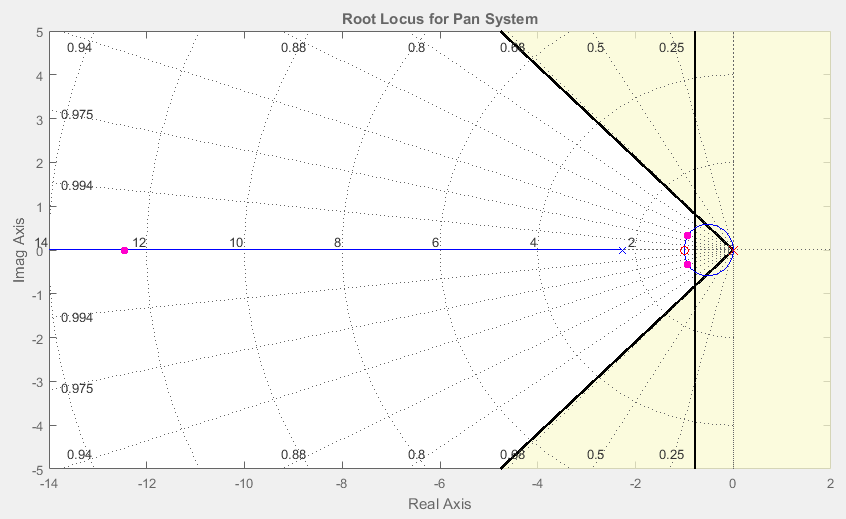
\includegraphics[scale=0.45]{Billeder/Pan_Rlocus.PNG}
	\end{center}
\caption{Her ses root locus plottet for vores pan-system med en PID-controller med $K_{P}=2$, $K_{I}=1$, $K_{D}=1$ og et gain på 0.01}
\label{fig:Pan_rlocus}
\end{figure}

\subsection{Gain}

Det sidste skridt er at bestemme et passende gain, så den endelige respons for systemerne tilfredsstiller projektets krav. De vigtigste ting at tage højde for er settling time, overshoot og hvor hårdt der reguleres med systemet. Hvis motorerne trækker for hårdt i rammerne kan bælterne kamme over og remskiverne kan rotere en lille smule på akslerne, da de bare er klemt fast med en sætskrue. 

Med kameraet monteret er den statiske friktion i systemet ret stor, samtig med at denne bidrager med et stort inertimoment der modvirker acceleration. Derfor er det svært at flytte systemet, når fejlen er meget lille. For at komme ud over denne begrænsning kan man øge gain'et for systemet. Det har dog den bivirkning at systemet regulerer meget kraftigt. En måde at forhindre denne situation er at sætte en øvre grænse for hvilken duty cycle, der må reguleres med. Dette gør systemet langsommere, men så længe settling time stadigvæk er under de 5 sekunder gør det ikke noget, da dette er vores krav til systemet.

Ud fra root locus plottet bestemmes et gain, der tages udgangspunkt i. Et gain på 0.005 til tilt-systemet giver et respons som på figur \ref{fig:Ideal_Response_Tilt}, og et gain på 0.008 til pan-systemet giver responset på figur \ref{fig:Ideal_Response_Pan}. 

\begin{figure}[t!]
    \centering
    \begin{subfigure}[t]{0.49\textwidth}
     \centering
        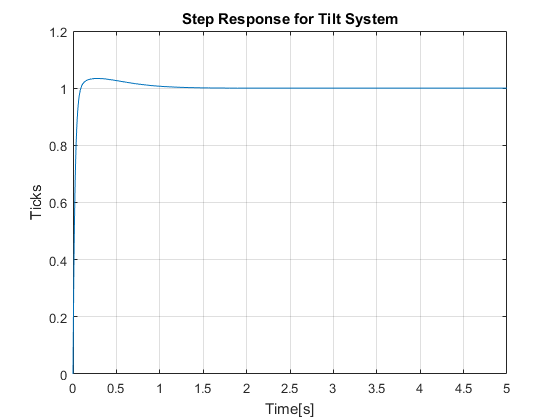
\includegraphics[width=1\textwidth]{Billeder/Ideal_Response_Tilt.png}
        \caption{Her ses responsen for tilt-systemet med et gain på 0.005}
        \label{fig:Ideal_Response_Tilt}
    \end{subfigure}
    \begin{subfigure}[t]{0.49\textwidth}
     \centering
        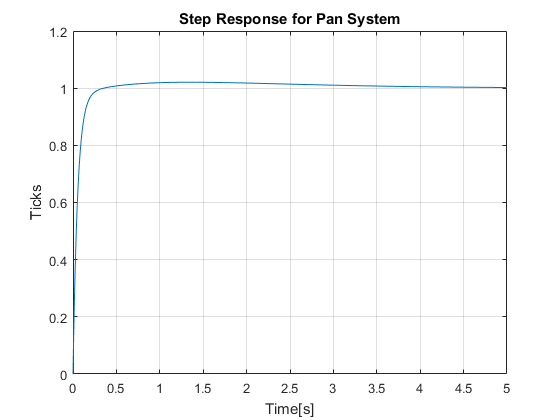
\includegraphics[width=1\textwidth]{Billeder/Ideal_Response_Pan.PNG}
        \caption{Her ses responsen for pan-systemet med et gain på 0.008}
        \label{fig:Ideal_Response_Pan}
    \end{subfigure}
    \caption{Her ses det ideelle step respons for systemerne}
\end{figure}

\subsubsection{Justering af Gain}

For at finde et gain, der kan bruges til små justeringer, ned til et tick, øges gain'et lidt efter lidt indtil systemet opfører sig som ønket under forsøg. Den øvre grænse for duty cyclen sættes også ned løbende, indtil systemet ikke regulerer for hårdt længere. Når der er fundet passende værdier til både gain og duty cycle-grænse, simuleres systemet igen i simulink, for at se om projektmålene stadigvæk overholdes. Forsøgene viste at gain'et helst skulle være større end 0.13 for at systemet kunne bevæge sig et tick ad gangen indenfor 5 sekunder. På figur \ref{fig:Simulated_Tilt}, \ref{fig:Measured_Tilt}, \ref{fig:Simulated_Pan} og \ref{fig:Measured_Pan} kan man se sammenligningen mellem simuleringen og målinger fra 0 til 540 ticks.

\begin{figure}[t!]
    \centering
    \begin{subfigure}[t]{0.8\textwidth}
     \centering
        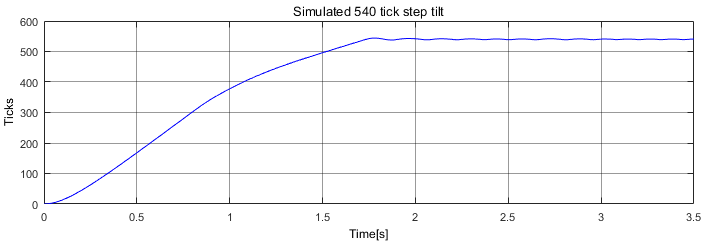
\includegraphics[width=1\textwidth]{Billeder/Simulated_Response_Tilt.png}
        \caption{Her ses det simulerede respons til tilt-systemet fra simulink}
        \label{fig:Simulated_Tilt}
    \end{subfigure}
    \begin{subfigure}[b]{0.8\textwidth}
     \centering
        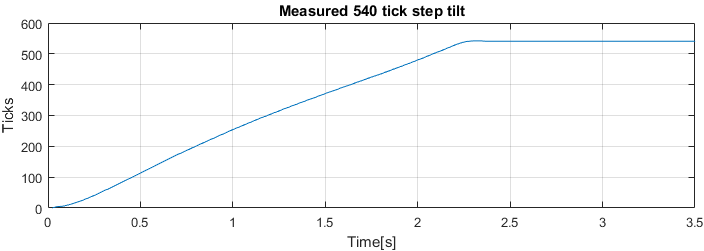
\includegraphics[width=1\textwidth]{Billeder/Measured_Response_Tilt.PNG}
        \caption{Her ses det målte respons fra tilt-systemet fra 0 til 90 grader}
        \label{fig:Measured_Tilt}
    \end{subfigure}
    \caption{Her ses sammenligningen af det simulerede og det målte tilt-system, ved et gain på 0.13 og en maximum duty cycle på 39 $\%$}
\end{figure}

Afvigelserne imellem de simulerede og de målter responser kan skyldes at systemet er simuleret som om det var kontinuert, ligesom at der i PID-blokken fra Simulink bruges et filter til differentieringsledet. Den endelige konfiguration kan ses i tabel \ref{tab:Results}.

\begin{figure}[t!]
    \centering
    \begin{subfigure}[t]{0.8\textwidth}
     \centering
        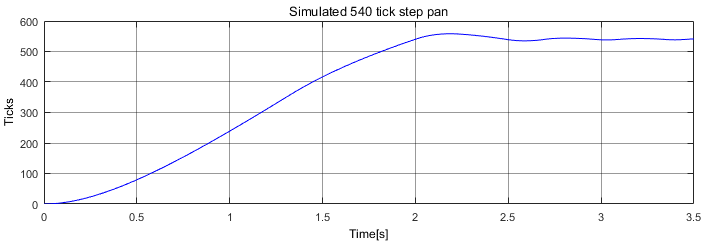
\includegraphics[width=1\textwidth]{Billeder/Simulated_Response_Pan.png}
        \caption{Her ses det simulerede respons til pan-systemet fra simulink}
        \label{fig:Simulated_Pan}
    \end{subfigure}
    \begin{subfigure}[b]{0.8\textwidth}
     \centering
        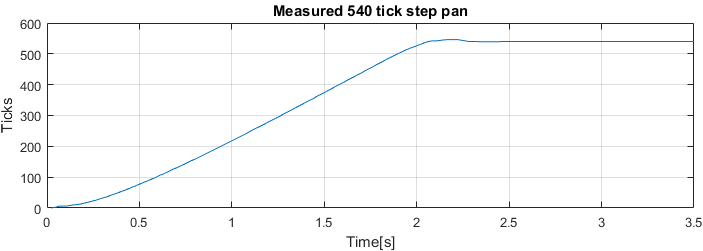
\includegraphics[width=1\textwidth]{Billeder/Measured_Response_Pan.PNG}
        \caption{Her ses det målte respons fra pan-systemet fra 0 til 90 grader}
        \label{fig:Measured_Pan}
    \end{subfigure}
    \caption{Her ses det ideelle step respons for systemerne}
\end{figure}

Simuleringen er lavet i simulink med og kan ses på figur \ref{fig:Simulink}. For at simulere at duty cyclen er låst fra 16 til 39 $\%$ skiftes der imellem to PID-controllere med de samme konstanter, der henholdsvis så er låst i intervallerne $0.16$ til $0.39$ og $-0.16$ til $-0.39$. Dette skift laves så, når fejlen $E(s)$ skifter fortegn.

\begin{figure}
\centering
        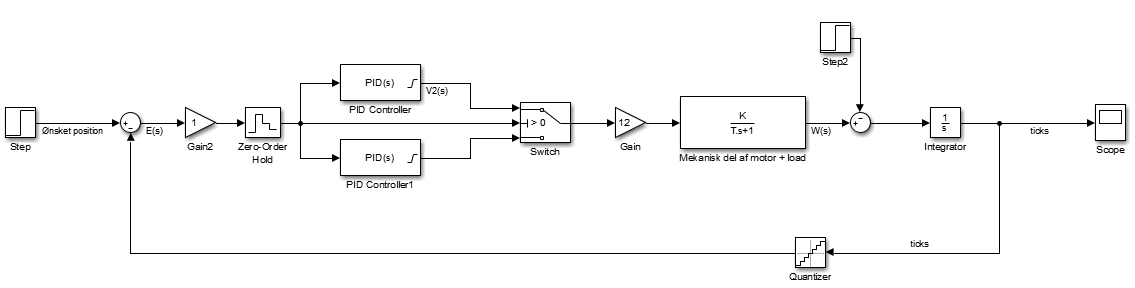
\includegraphics[width=1\textwidth]{Billeder/Simulink.PNG}
        \caption{Her ses blokdiagrammet for kontrolsystemet i simulink.}
        \label{fig:Simulink}
\end{figure}

\begin{table}[]
\centering
\caption{Her ses den endelige konfiguration af systemet}
\label{tab:Results}
\begin{tabular}{|l|l|l|l|l|l|l|}
\hline
     & $K_{P}$ & $K_{I}$ & $K_{D}$ & Gain & DC min & DC max \\ \hline
Tilt & 8  & 16 & 1  & 0.13 & 16\%   & 39\%   \\ \hline
Pan  & 2  & 1  & 1  & 0.13 & 16\%   & 39\%   \\ \hline
\end{tabular}
\end{table}